%!TEX root = paper/paper.tex
\subsection{Application: Style-Based Image Search}

\newcommand{\fgap}{.6in}
\begin{figure}[h!]
\centering
\begin{tabular}{m{.02in}|m{\fgap} m{\fgap} m{\fgap} m{\fgap} m{\fgap}}
    \begin{turn}{90}\footnotesize{Minimal}\end{turn} &
    
\includegraphics[width=.75in]{../../figures/flickr_on_flickr/pred_style_Minimal/w/0.jpg} &
    
\includegraphics[width=.75in]{../../figures/flickr_on_flickr/pred_style_Minimal/w/1.jpg} &
    
\includegraphics[width=.75in]{../../figures/flickr_on_flickr/pred_style_Minimal/w/2.jpg} &
    
\includegraphics[width=.75in]{../../figures/flickr_on_flickr/pred_style_Minimal/w/3.jpg} &
    
\includegraphics[width=.75in]{../../figures/flickr_on_flickr/pred_style_Minimal/w/4.jpg} \\
    \begin{turn}{90}\footnotesize{Melancholy}\end{turn} &
    
\includegraphics[width=.75in]{../../figures/flickr_on_flickr/pred_style_Melancholy/w/0.jpg} &
    
\includegraphics[width=.75in]{../../figures/flickr_on_flickr/pred_style_Melancholy/w/1.jpg} &
    
\includegraphics[width=.75in]{../../figures/flickr_on_flickr/pred_style_Melancholy/w/2.jpg} &
    
\includegraphics[width=.75in]{../../figures/flickr_on_flickr/pred_style_Melancholy/w/3.jpg} &
    
\includegraphics[width=.75in]{../../figures/flickr_on_flickr/pred_style_Melancholy/w/4.jpg} \\
    \begin{turn}{90}\footnotesize{HDR}\end{turn} &
    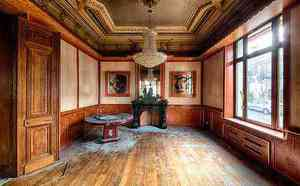
\includegraphics[width=.75in]{../../figures/flickr_on_flickr/pred_style_HDR/w/0.jpg} &
    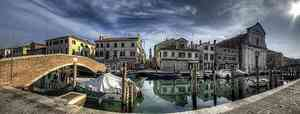
\includegraphics[width=.75in]{../../figures/flickr_on_flickr/pred_style_HDR/w/1.jpg} &
    
\includegraphics[width=.75in]{../../figures/flickr_on_flickr/pred_style_HDR/w/2.jpg} &
    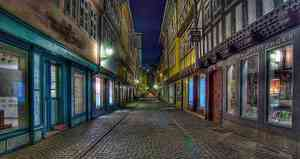
\includegraphics[width=.75in]{../../figures/flickr_on_flickr/pred_style_HDR/w/3.jpg} &
    
\includegraphics[width=.75in]{../../figures/flickr_on_flickr/pred_style_HDR/w/4.jpg} \\
    \begin{turn}{90}\footnotesize{Vintage}\end{turn} &
    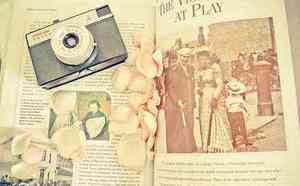
\includegraphics[width=.75in]{../../figures/flickr_on_flickr/pred_style_Vintage/w/0.jpg} &
    
\includegraphics[width=.75in]{../../figures/flickr_on_flickr/pred_style_Vintage/w/1.jpg} &
    
\includegraphics[width=.75in]{../../figures/flickr_on_flickr/pred_style_Vintage/w/2.jpg} &
    
\includegraphics[width=.75in]{../../figures/flickr_on_flickr/pred_style_Vintage/w/3.jpg} &
    
\includegraphics[width=.75in]{../../figures/flickr_on_flickr/pred_style_Vintage/w/4.jpg} \\
\end{tabular}
\vspace{1em}
\caption{
    Top five most-confident positive predictions on the Flickr Style test set, for a few different styles.
    See Figures 1-3 of the Supplemental Material for more results.
}\label{fig:flickr_on_flickr}
\end{figure}


Style classifiers learned on our datasets can be used toward novel goals.
For example, sources of stock photography or design inspiration may be better navigated with a vocabulary of style.
Currently, companies expend labor to manually annotate stock photography with such labels.
With our approach, any image collection can be searchable and rankable by style.

To demonstrate, we apply our Flickr-learned style classifiers to a new dataset of 80K images gathered on Pinterest (also available with our code release); some results are shown in \autoref{fig:flickr_on_pinterest}.
Interestingly, styles learned from photographs can be used to order paintings, and styles learned from paintings can be used to order photographs, as illustrated in \autoref{fig:photo_painting}.

\begin{figure*}[ht]
\centering
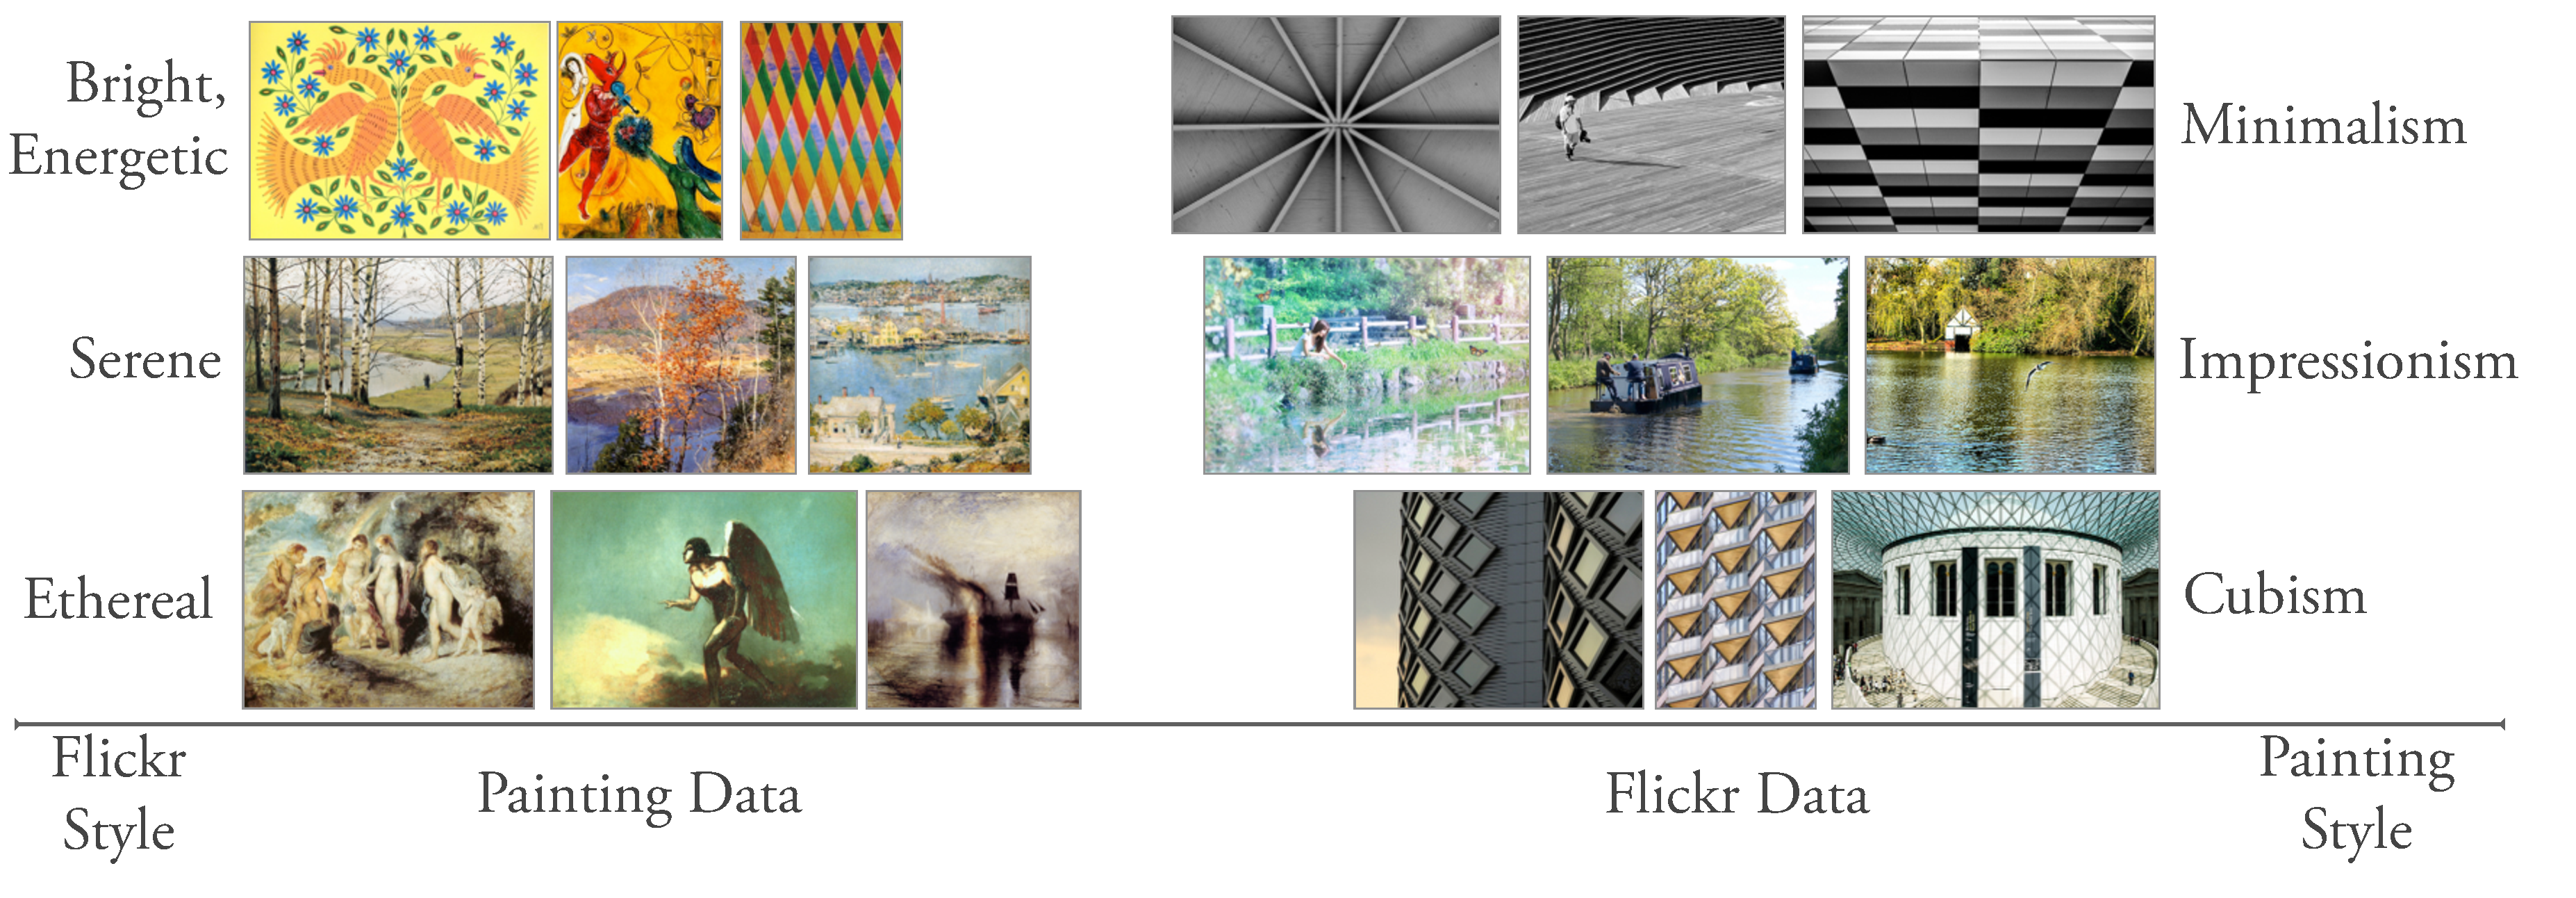
\includegraphics[width=.95\linewidth]{../../figures/style_by_style.pdf}
\vspace{-1ex}
\caption{
    Cross-dataset style.
    On the left are shown top scorers from the Wikipaintings set, for styles learned on the Flickr set.
    On the right, Flickr photographs are accordingly sorted by Painting style.
    (Figure best viewed in color.)
}
\label{fig:photo_painting}
\end{figure*}

\newcommand{\dgap}{.42in}
\begin{figure}
\begin{subfigure}[t]{0.48\linewidth}
    \begin{tabular}{m{.02in}|m{\dgap} m{\dgap} m{\dgap}}
    \begin{turn}{90}\small{Bright}\end{turn} &
    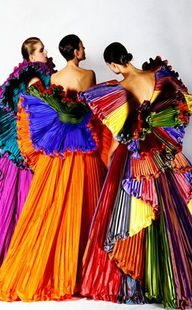
\includegraphics[width=.53in]{../../figures/flickr_on_pinterest/dress/pred_style_Bright/h/0.jpg} &
    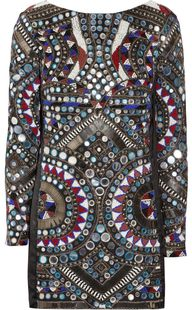
\includegraphics[width=.53in]{../../figures/flickr_on_pinterest/dress/pred_style_Bright/h/1.jpg} &
    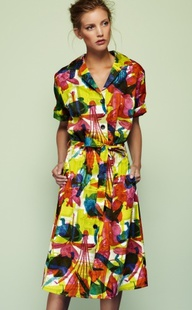
\includegraphics[width=.53in]{../../figures/flickr_on_pinterest/dress/pred_style_Bright/h/2.jpg} \\ \\
    \begin{turn}{90}\small{Pastel}\end{turn} &
    
\includegraphics[width=.53in]{../../figures/flickr_on_pinterest/dress/pred_style_Pastel/h/0.jpg} &
    
\includegraphics[width=.53in]{../../figures/flickr_on_pinterest/dress/pred_style_Pastel/h/1.jpg} &
    
\includegraphics[width=.53in]{../../figures/flickr_on_pinterest/dress/pred_style_Pastel/h/2.jpg} \\ \\
    \begin{turn}{90}\small{Ethereal}\end{turn} &
    
\includegraphics[width=.53in]{../../figures/flickr_on_pinterest/dress/pred_style_Ethereal/h/0.jpg} &
    
\includegraphics[width=.53in]{../../figures/flickr_on_pinterest/dress/pred_style_Ethereal/h/1.jpg} &
    
\includegraphics[width=.53in]{../../figures/flickr_on_pinterest/dress/pred_style_Ethereal/h/2.jpg} \\ \\
    \begin{turn}{90}\small{Noir}\end{turn} &
    
\includegraphics[width=.53in]{../../figures/flickr_on_pinterest/dress/pred_style_Noir/h/0.jpg} &
    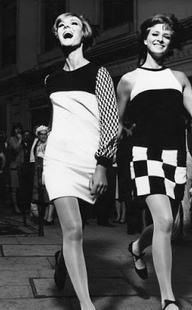
\includegraphics[width=.53in]{../../figures/flickr_on_pinterest/dress/pred_style_Noir/h/1.jpg} &
    
\includegraphics[width=.53in]{../../figures/flickr_on_pinterest/dress/pred_style_Noir/h/2.jpg} \\ \\
    \begin{turn}{90}\small{Vintage}\end{turn} &
    
\includegraphics[width=.53in]{../../figures/flickr_on_pinterest/flower/pred_style_Vintage/h/0.jpg} &
    
\includegraphics[width=.53in]{../../figures/flickr_on_pinterest/flower/pred_style_Vintage/h/2.jpg} &
    
\includegraphics[width=.53in]{../../figures/flickr_on_pinterest/flower/pred_style_Vintage/h/3.jpg} \\
    \end{tabular}
    \caption{Query: ``dress''.}
\end{subfigure}\hfill%
\begin{subfigure}[t]{0.48\linewidth}
    \begin{tabular}{m{.02in}|m{\dgap} m{\dgap} m{\dgap}}
    \begin{turn}{90}\small{DoF}\end{turn} &
    
\includegraphics[width=.53in]{../../figures/flickr_on_pinterest/flower/pred_style_Depth_of_Field/h/1.jpg} &
    
\includegraphics[width=.53in]{../../figures/flickr_on_pinterest/flower/pred_style_Depth_of_Field/h/3.jpg} &
    
\includegraphics[width=.53in]{../../figures/flickr_on_pinterest/flower/pred_style_Depth_of_Field/h/4.jpg} \\ \\
    \begin{turn}{90}\small{Romantic}\end{turn} &
    
\includegraphics[width=.53in]{../../figures/flickr_on_pinterest/flower/pred_style_Romantic/h/0.jpg} &
    
\includegraphics[width=.53in]{../../figures/flickr_on_pinterest/flower/pred_style_Romantic/h/1.jpg} &
    
\includegraphics[width=.53in]{../../figures/flickr_on_pinterest/flower/pred_style_Romantic/h/3.jpg} \\ \\
    \begin{turn}{90}\small{Sunny}\end{turn} &
    
\includegraphics[width=.53in]{../../figures/flickr_on_pinterest/flower/pred_style_Sunny/h/0.jpg} &
    
\includegraphics[width=.53in]{../../figures/flickr_on_pinterest/flower/pred_style_Sunny/h/1.jpg} &
    
\includegraphics[width=.53in]{../../figures/flickr_on_pinterest/flower/pred_style_Sunny/h/2.jpg} \\ \\
    \begin{turn}{90}\small{Geometric}\end{turn} &
    
\includegraphics[width=.53in]{../../figures/flickr_on_pinterest/flower/pred_style_Geometric_Composition/h/0.jpg} &
    
\includegraphics[width=.53in]{../../figures/flickr_on_pinterest/flower/pred_style_Geometric_Composition/h/1.jpg} &
    
\includegraphics[width=.53in]{../../figures/flickr_on_pinterest/flower/pred_style_Geometric_Composition/h/4.jpg} \\ \\
    \begin{turn}{90}\small{Serene}\end{turn} &
    
\includegraphics[width=.53in]{../../figures/flickr_on_pinterest/flower/pred_style_Serene/h/0.jpg} &
    
\includegraphics[width=.53in]{../../figures/flickr_on_pinterest/flower/pred_style_Serene/h/2.jpg} &
    \includegraphics[width=.53in]{../../figures/flickr_on_pinterest/flower/pred_style_Serene/h/3.jpg} \\
    \end{tabular}
    \caption{Query: ``flower''.}
\end{subfigure}
\\
\caption{
    Example of filtering image search results by style.
    Our Flickr Style classifiers are applied to images found on Pinterest.
    The images are searched by the text contents of their captions, then filtered by the response of the style classifiers.
    Here we show three out of top five results for different query/style combinations.
}\label{fig:flickr_on_pinterest}
\end{figure}

